\documentclass[t]{beamer}
%\documentclass[finnish,english,handout]{beamer}

% Uncomment if want to show notes
% \setbeameroption{show notes}

\mode<presentation>
{
%  \usetheme{Copenhagen}
  % oder ...
  
  %\setbeamercovered{transparent}
  % oder auch nicht
}
\setbeamertemplate{itemize items}[circle]
\setbeamercolor{frametitle}{bg=white,fg=navyblue}



\usepackage[T1]{fontenc}
\usepackage[latin1]{inputenc}
\usepackage{times}
\usepackage{epic,epsfig}
\usepackage{subfigure,float}
\usepackage{amsmath,amsfonts,amssymb}
\usepackage{inputenc}
\usepackage{afterpage}
\usepackage{url}
\urlstyle{same}
\usepackage{amsbsy}
\usepackage{eucal}
\usepackage{rotating}
\usepackage{listings}
\usepackage{lstbayes}
\usepackage[all,poly,ps,color]{xy}
\usepackage{eurosym}
\usepackage{microtype}

\usepackage{natbib}
\bibliographystyle{apalike}

\hypersetup{%
  bookmarksopen=true,
  bookmarksnumbered=true,
  pdftitle={Stan},
  pdfsubject={Bayesian data analysis},
  pdfauthor={Aki Vehtari},
  pdfkeywords={},
  pdfstartview={FitH -32768},
  colorlinks=true,
  linkcolor=navyblue,
  citecolor=navyblue,
  filecolor=navyblue,
  urlcolor=navyblue
}

% \definecolor{hutblue}{rgb}{0,0.2549,0.6784}
% \definecolor{midnightblue}{rgb}{0.0977,0.0977,0.4375}
% \definecolor{hutsilver}{rgb}{0.4863,0.4784,0.4784}
% \definecolor{lightgray}{rgb}{0.95,0.95,0.95}
% \definecolor{section}{rgb}{0,0.2549,0.6784}
% \definecolor{list1}{rgb}{0,0.2549,0.6784}
\definecolor{forestgreen}{rgb}{0.1333,0.5451,0.1333}
\definecolor{navyblue}{rgb}{0,0,0.5}
\renewcommand{\emph}[1]{\textcolor{navyblue}{#1}}

\graphicspath{{./figs/}}

\pdfinfo{            
  /Title      (Bayesian data analysis 4)
  /Author     (Aki Vehtari) % 
  /Keywords   (Bayesian probability theory, Bayesian inference, Bayesian data analysis)
}


\parindent=0pt
\parskip=8pt
\tolerance=9000
\abovedisplayshortskip=0pt

\setbeamertemplate{navigation symbols}{}
\setbeamertemplate{headline}[default]{}
\setbeamertemplate{headline}[text line]{\insertsection}
\setbeamertemplate{footline}[frame number]


\def\o{{\mathbf o}}
\def\t{{\mathbf \theta}}
\def\w{{\mathbf w}}
\def\x{{\mathbf x}}
\def\y{{\mathbf y}}
\def\z{{\mathbf z}}

\DeclareMathOperator{\E}{E}
\DeclareMathOperator{\Var}{Var}
\DeclareMathOperator{\var}{var}
\DeclareMathOperator{\Sd}{Sd}
\DeclareMathOperator{\sd}{sd}
\DeclareMathOperator{\Gammad}{Gamma}
\DeclareMathOperator{\Invgamma}{Inv-gamma}
\DeclareMathOperator{\Bin}{Bin}
\DeclareMathOperator{\Negbin}{Neg-bin}
\DeclareMathOperator{\Poisson}{Poisson}
\DeclareMathOperator{\Beta}{Beta}
\DeclareMathOperator{\logit}{logit}
\DeclareMathOperator{\N}{N}
\DeclareMathOperator{\U}{U}
\DeclareMathOperator{\BF}{BF}
\DeclareMathOperator{\Invchi2}{Inv-\chi^2}
\DeclareMathOperator{\NInvchi2}{N-Inv-\chi^2}
\DeclareMathOperator{\InvWishart}{Inv-Wishart}
\DeclareMathOperator{\tr}{tr}
% \DeclareMathOperator{\Pr}{Pr}
\def\euro{{\footnotesize \EUR\, }}
\DeclareMathOperator{\rep}{\mathrm{rep}}



\title[]{Bayesian data analysis}
\subtitle{}

\author{Aki Vehtari}

\institute[Aalto]{}


\begin{document} 

\begin{frame}{Common statistical tests as Bayesian models}

  \begin{itemize}
  \item Most common statistical tests are linear models\\
    \vspace{0.5\baselineskip}
    \hspace{-0.8cm}\begin{minipage}[t]{1.0\linewidth}
      {\small
        \begin{tabular}{lll}
          $t$-test & mean of data & {\tt stan\_glm(y \~\ 1)}\\
          paired $t$-test & mean of diffs &{\tt stan\_glm((y1 - y2) \~\  1)}\\
          Pearson correl. & linear model &{\tt stan\_glm(y \~\  1 + x)}\\
          two-sample $t$-test & group means &{\tt stan\_glm(y \~\  1 + gid)}\\
          ANOVA & hier. model &{\tt stan\_glm(y \~\  1 + (1 | gid))}\\
          $\ldots$ &
        \end{tabular}}
      \end{minipage}
  \item<2->  Possible to extend, e.g., with group specific variances and and
    different distributions such $t$- or Poisson distribution
    \begin{itemize}
    \item and go beyond named tests
    \end{itemize}
  \item<3-> See longer list and illustrations (with {\tt lm}) at
  \url{https://lindeloev.github.io/tests-as-linear/}\\
  and\\
  with rstanarm in \href{https://avehtari.github.io/ROS-Examples/}{Regression and other stories}
\end{itemize}

\end{frame}

\begin{frame}{Frequentist hypothesis testing}
  
  \begin{itemize}
  \item Frequentist approach can be used to to make estimates and
    confidence intervals, but for some reason null hypothesis testing
    has had a very big role
    \begin{itemize}
    \item<2-> reporting just the null hypothesis testing result throws
      away lot of useful information
    \item<3-> some Bayesians are also into null hypothesis testing
    \end{itemize}
  \item<4-> Frequentist null hypothesis testing
    \begin{itemize}
    \item asks what if data is generated from the smaller model
    \item doesn't tell whether the more complex model is good enough
    \end{itemize}
  \item<5-> Some frequentists are now advocating looking at intervals and
    equivalence testing
  \end{itemize}
  
\end{frame}

\begin{frame}{Bayesian hypothesis testing}

  \begin{itemize}
  \item Instead of hypothesis testing, report full posterior \only<1>{and}
    \begin{itemize}
      \only<1>{
      \item<1> compare to expert information
      \item<1> combine with utility/cost function
      }
      \only<2>{
      \item for continuous posterior there is zero probability that
        e.g. treatment effect is exactly zero
      }
      \only<3>{
      \item for continuous posterior we could compute the probability
        that we know the sign of the effect
      }
      \only<4>{
      \item for continuous posterior some people compare whether
        posterior interval includes null case
      }
    \end{itemize}
  \end{itemize}
  
  \only<1>{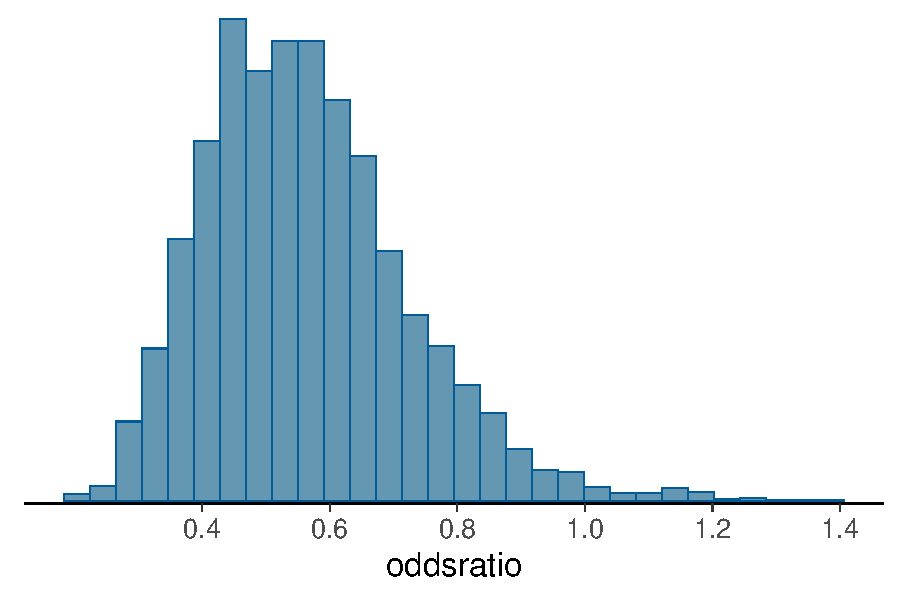
\includegraphics[width=10cm]{odds1_fullp.pdf}}
  \only<2>{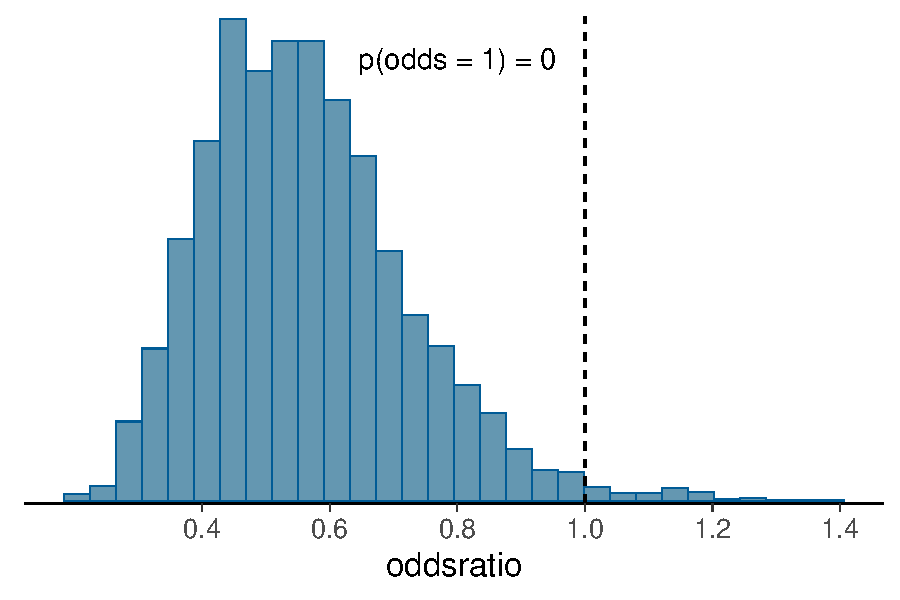
\includegraphics[width=10cm]{odds1_eq.pdf}}
  \only<3>{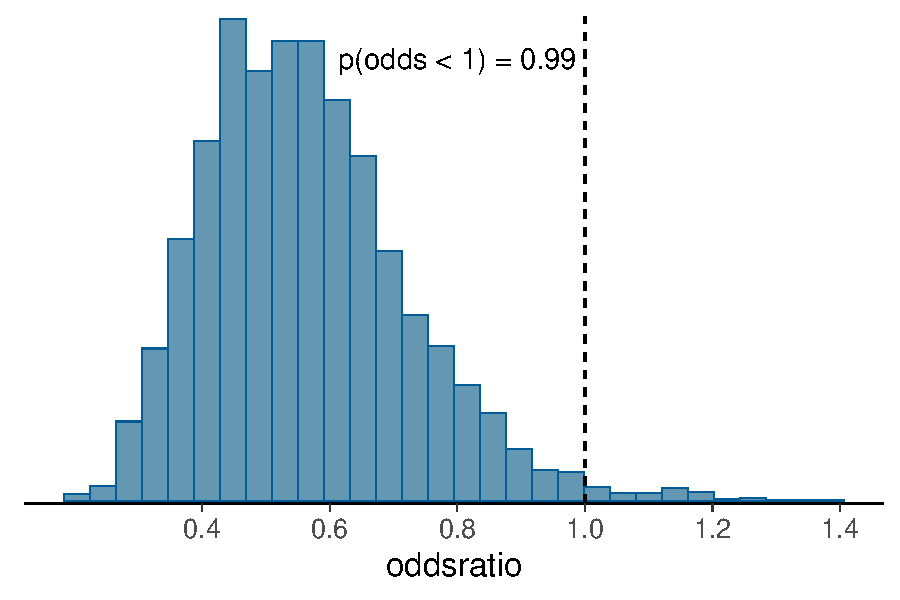
\includegraphics[width=10cm]{odds1_less.pdf}}
  \only<4>{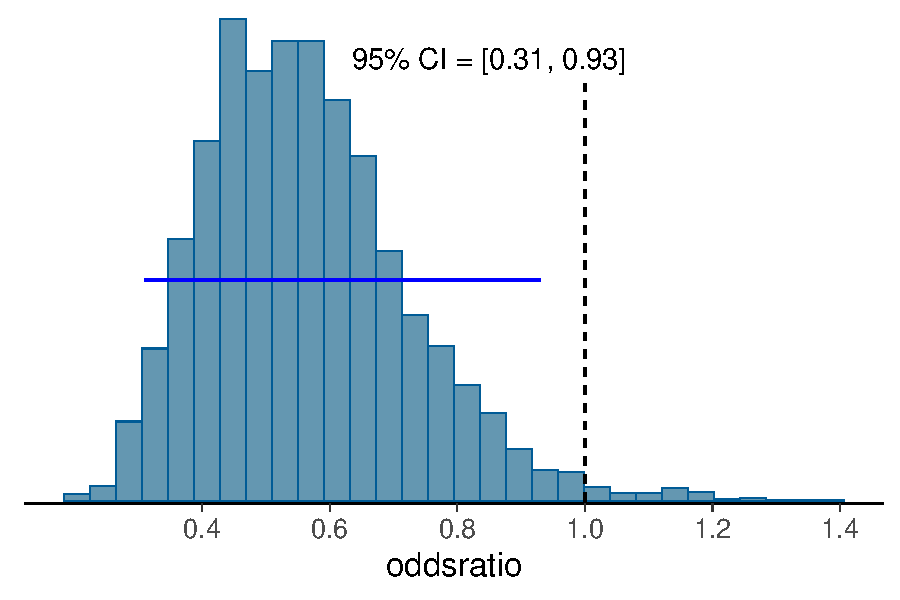
\includegraphics[width=10cm]{odds1_ci.pdf}}
  
\end{frame}

\begin{frame}{Bayesian hypothesis testing}

  \begin{itemize}
  \item Equivalence testing (region of practical equivalence)
    \begin{itemize}
      \only<1>{
    \item what is the probability that the effect is closer than
      $\epsilon$ to null, where $\epsilon$ is based on what is
      practically useful effect size
      }
      \only<2>{
      \item some people combine posterior interval and region of
        practical equivalence}
    \end{itemize}
  \end{itemize}

    \only<1>{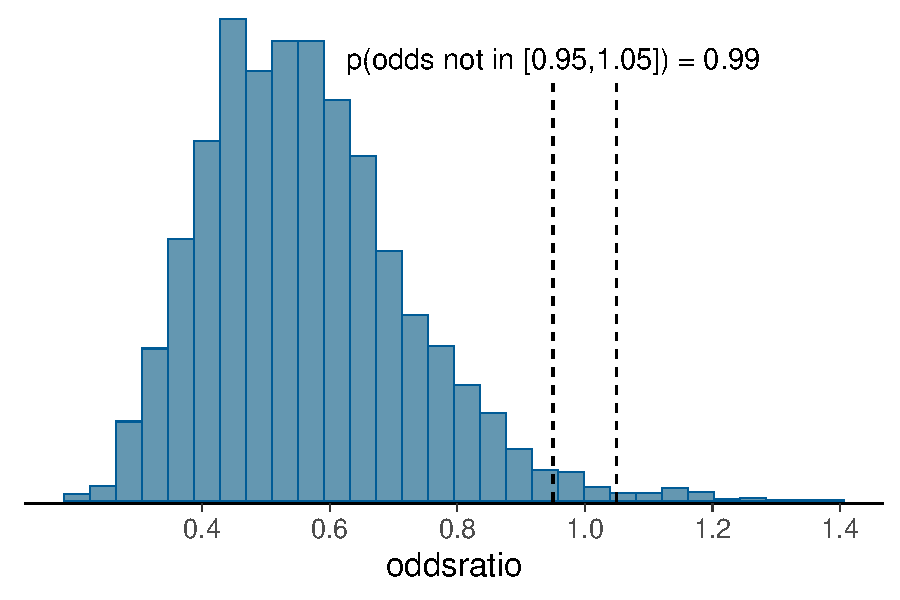
\includegraphics[width=10cm]{odds1_rope.pdf}}
    \only<2>{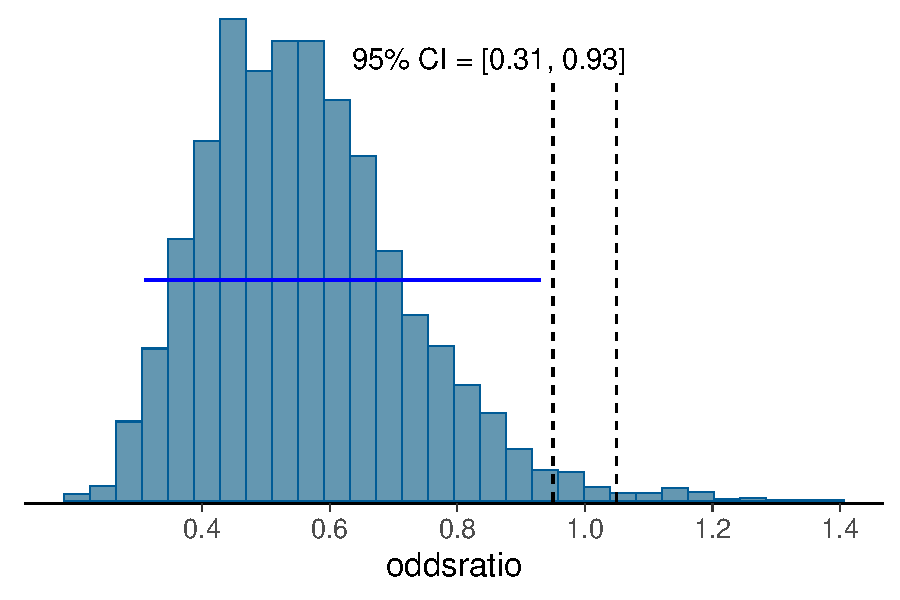
\includegraphics[width=10cm]{odds1_cirope.pdf}}

\end{frame}

\begin{frame}{Bayesian hypothesis testing}

  \begin{itemize}
  \item Instead of hypothesis testing, report full posterior
    \begin{itemize}
      \only<1>{
      \item for continuous posterior there is zero probability that
        e.g. treatment effect is exactly zero
      }
      \only<2>{
      \item for continuous posterior we could compute the probability
        that we know the sign of the effect
      }
      \only<3>{
      \item for continuous posterior some people compare whether
        posterior interval includes null case
      }
      \only<4->{
      \item region of practical equivalence (ROPE)\\
        \phantom{posterior interval includes null case}
      }
    \end{itemize}
  \end{itemize}
  
  \only<1>{\begin{minipage}{14.1cm}
      \hspace{-1.2cm}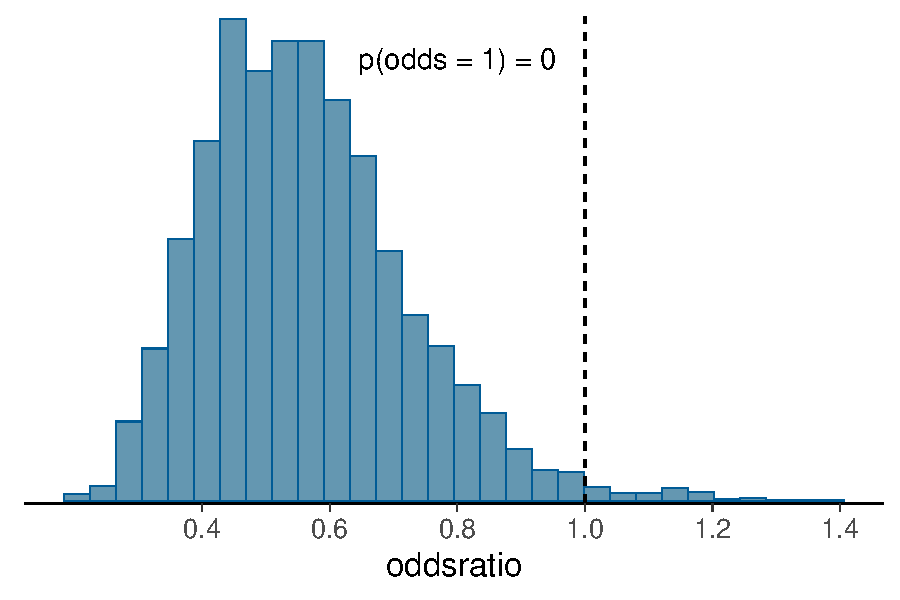
\includegraphics[width=6.8cm]{odds1_eq.pdf}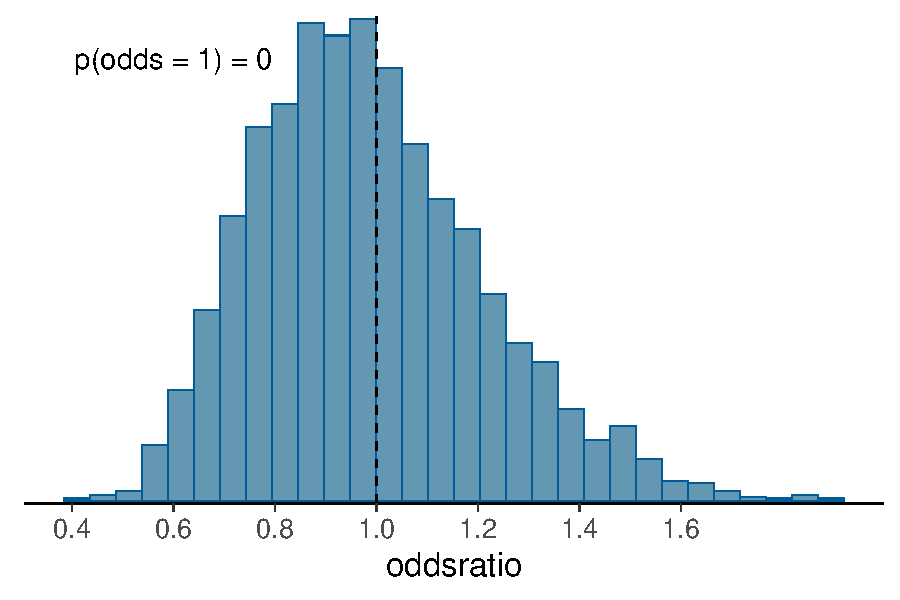
\includegraphics[width=6.8cm]{odds2_eq.pdf}
    \end{minipage}}
  \only<2>{\begin{minipage}{14.1cm}
      \hspace{-1.2cm}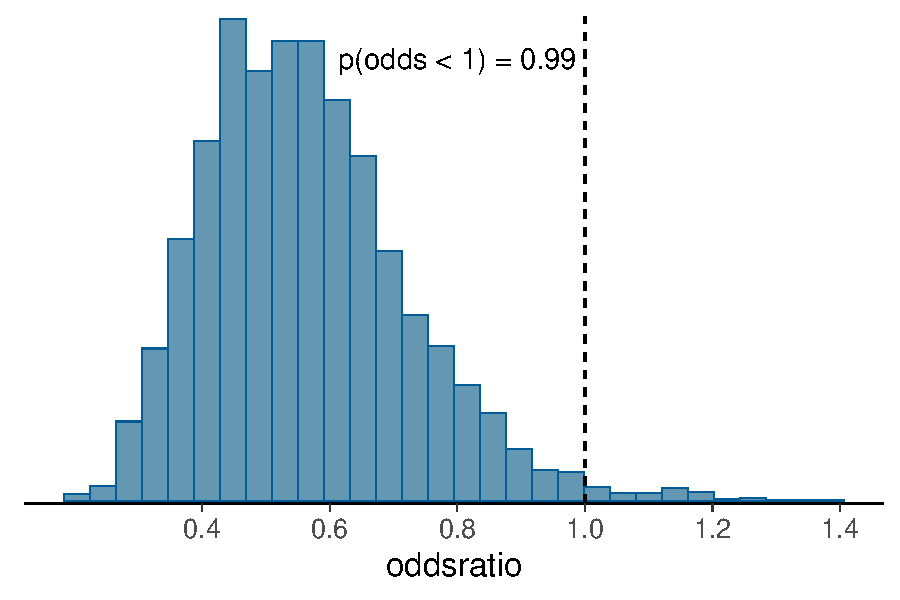
\includegraphics[width=6.8cm]{odds1_less.pdf}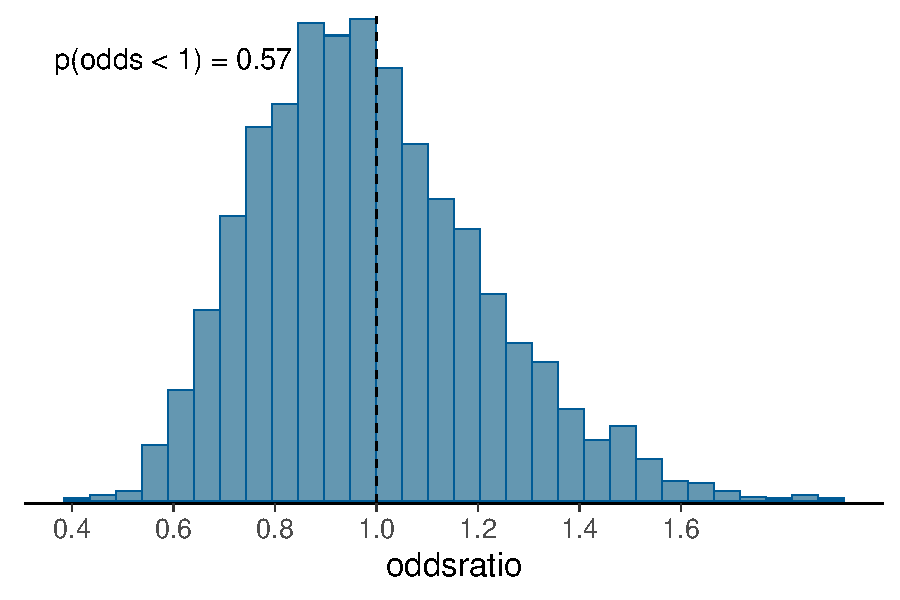
\includegraphics[width=6.8cm]{odds2_less.pdf}
    \end{minipage}}
  \only<3>{\begin{minipage}{14.1cm}
      \hspace{-1.2cm}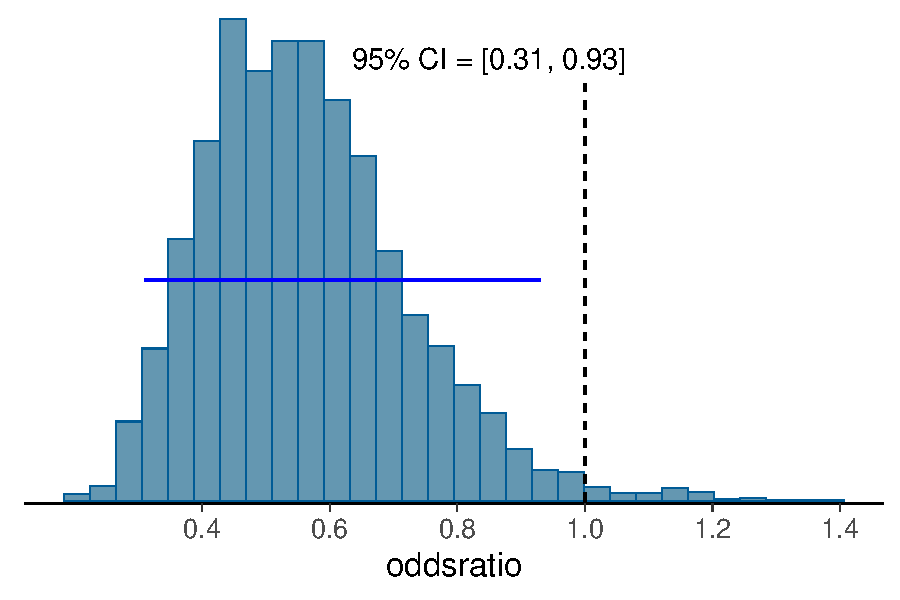
\includegraphics[width=6.8cm]{odds1_ci.pdf}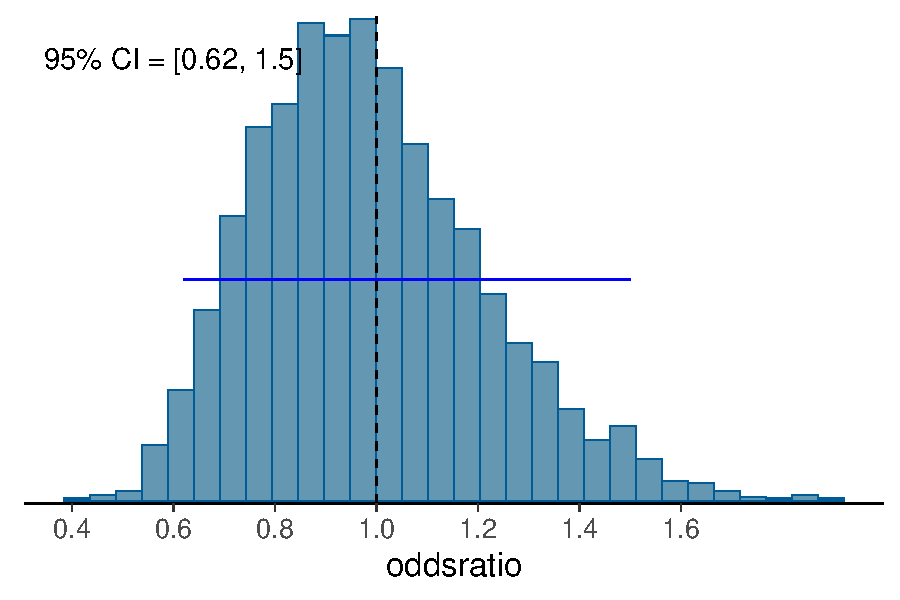
\includegraphics[width=6.8cm]{odds2_ci.pdf}
    \end{minipage}}
  \only<4>{\begin{minipage}{14.1cm}
      \hspace{-1.2cm}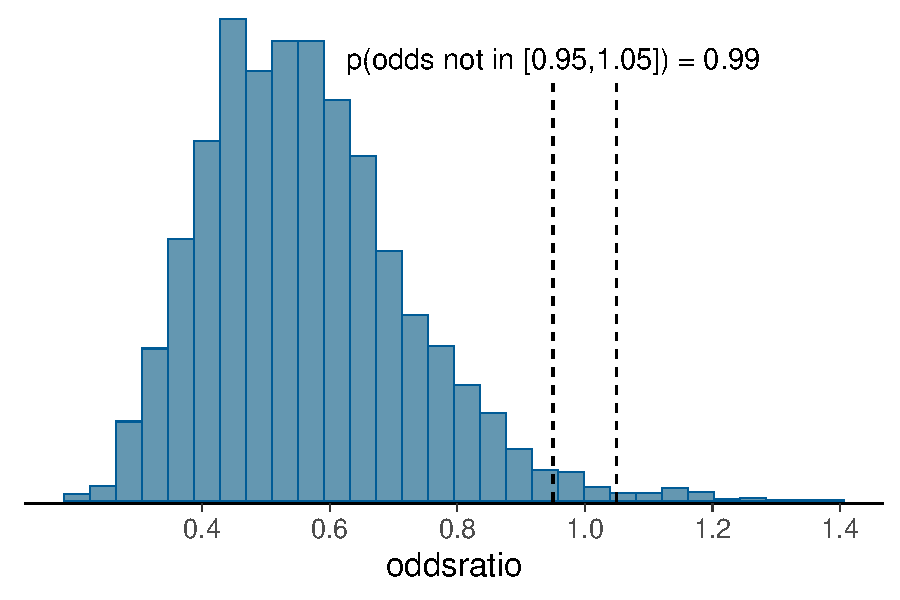
\includegraphics[width=6.8cm]{odds1_rope.pdf}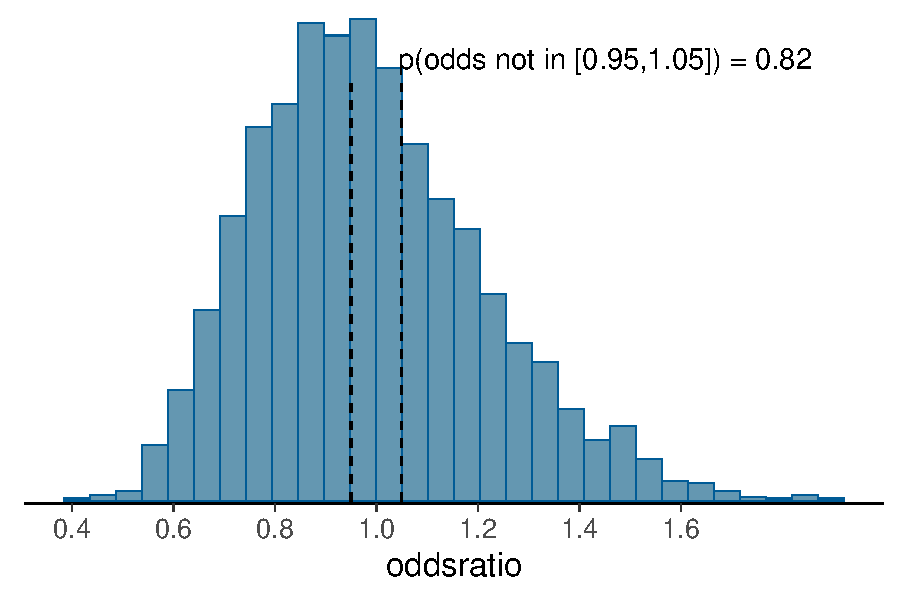
\includegraphics[width=6.8cm]{odds2_rope.pdf}
    \end{minipage}}
  \only<5>{\begin{minipage}{14.1cm}
      \hspace{-1.2cm}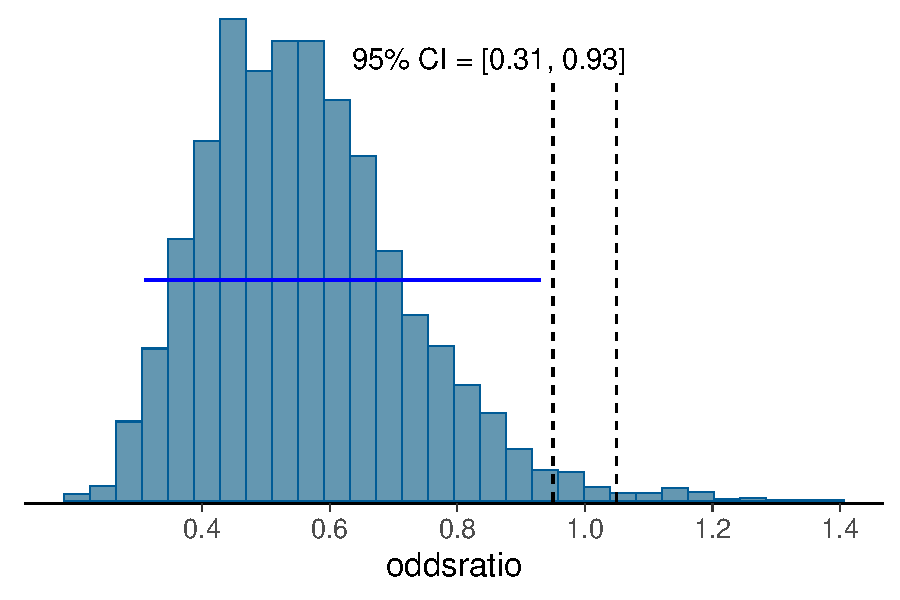
\includegraphics[width=6.8cm]{odds1_cirope.pdf}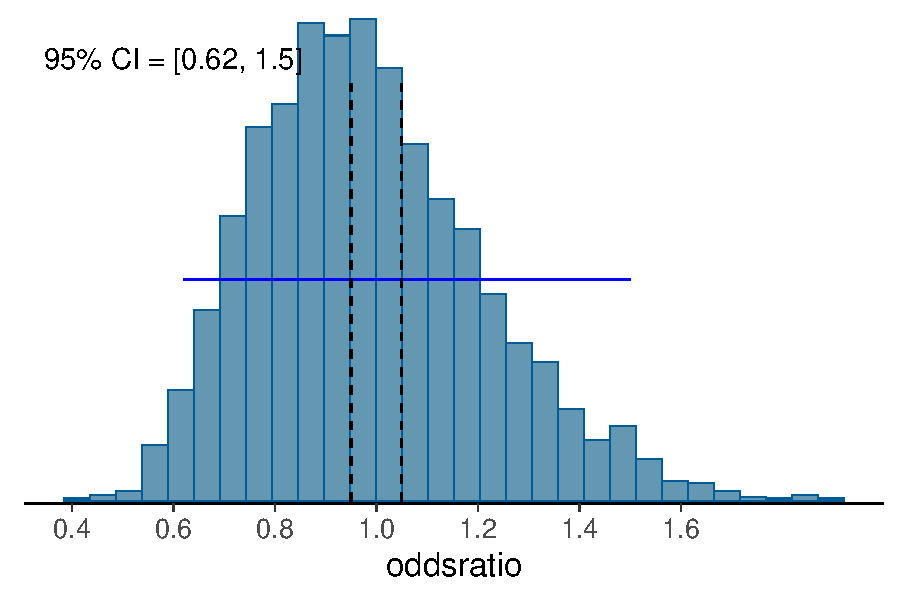
\includegraphics[width=6.8cm]{odds2_cirope.pdf}
    \end{minipage}}
  
\end{frame}

\begin{frame}{Bayesian hypothesis testing}

  \begin{itemize}
  \item Instead of hypothesis testing, report full posterior
    \begin{itemize}
      \only<1>{
      \item for continuous posterior there is zero probability that
        e.g. treatment effect is exactly zero
      }
      \only<2>{
      \item for continuous posterior we could compute the probability
        that we know the sign of the effect
      }
      \only<3>{
      \item for continuous posterior some people compare whether
        posterior interval includes null case
      }
      \only<4->{
      \item region of practical equivalence (ROPE)\\~
      }
    \end{itemize}
  \end{itemize}
  
  \only<2>{\begin{minipage}{14.1cm}
      \hspace{-1.2cm}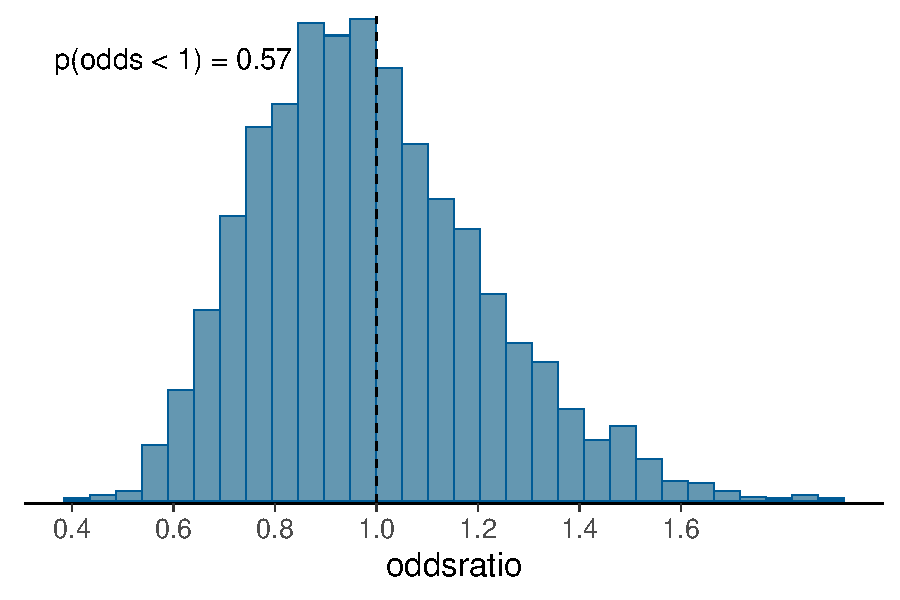
\includegraphics[width=6.8cm]{odds2_less.pdf}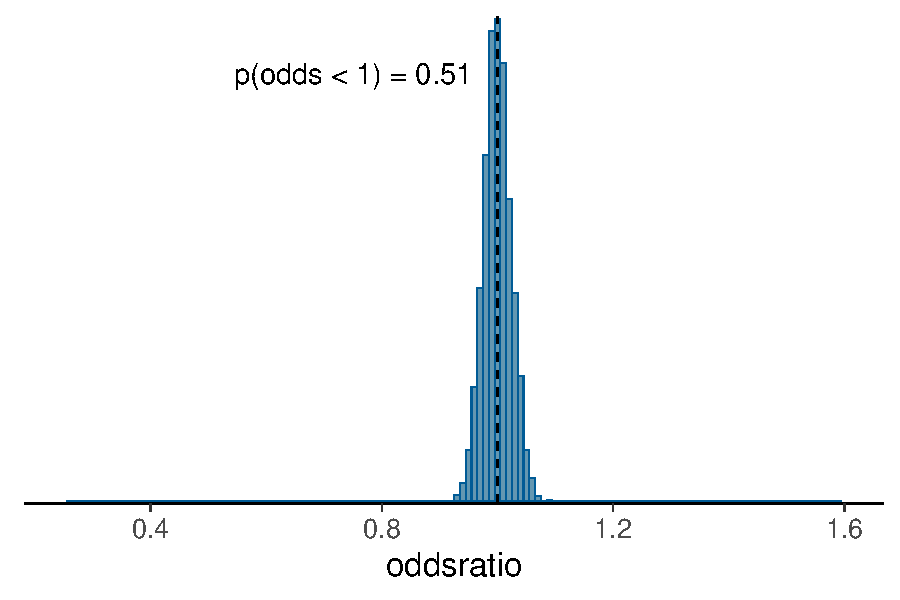
\includegraphics[width=6.8cm]{odds3_less.pdf}
    \end{minipage}}
  \only<3>{\begin{minipage}{14.1cm}
      \hspace{-1.2cm}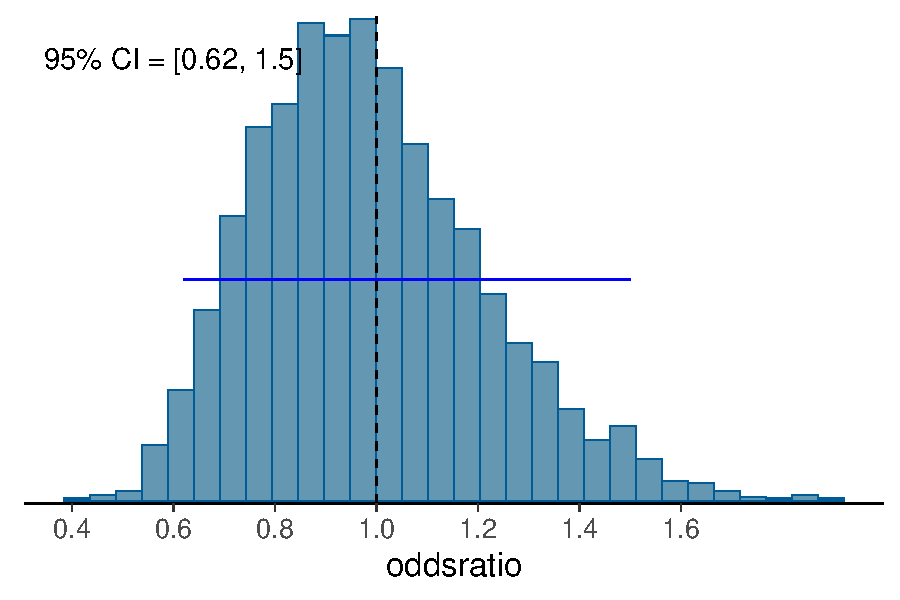
\includegraphics[width=6.8cm]{odds2_ci.pdf}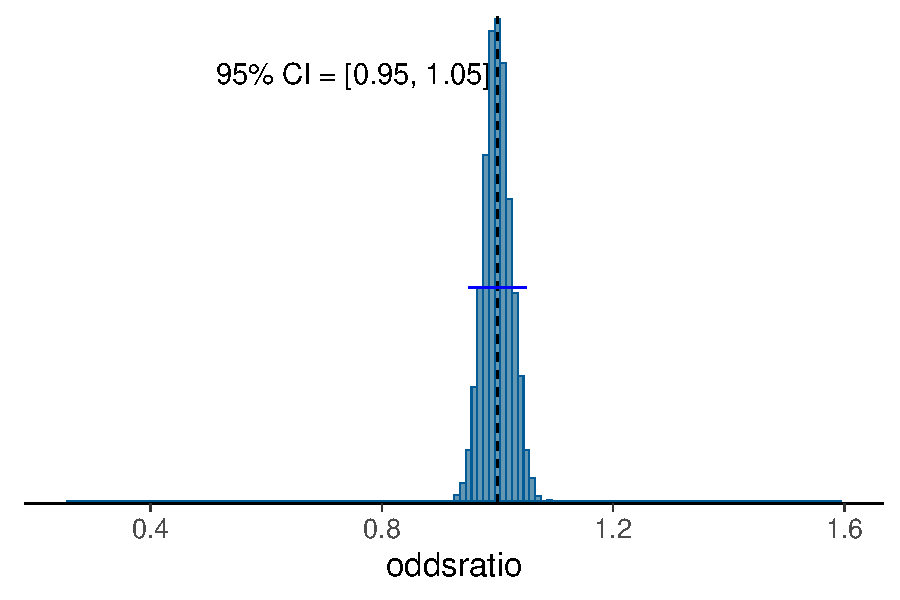
\includegraphics[width=6.8cm]{odds3_ci.pdf}
    \end{minipage}}
  \only<4>{\begin{minipage}{14.1cm}
      \hspace{-1.2cm}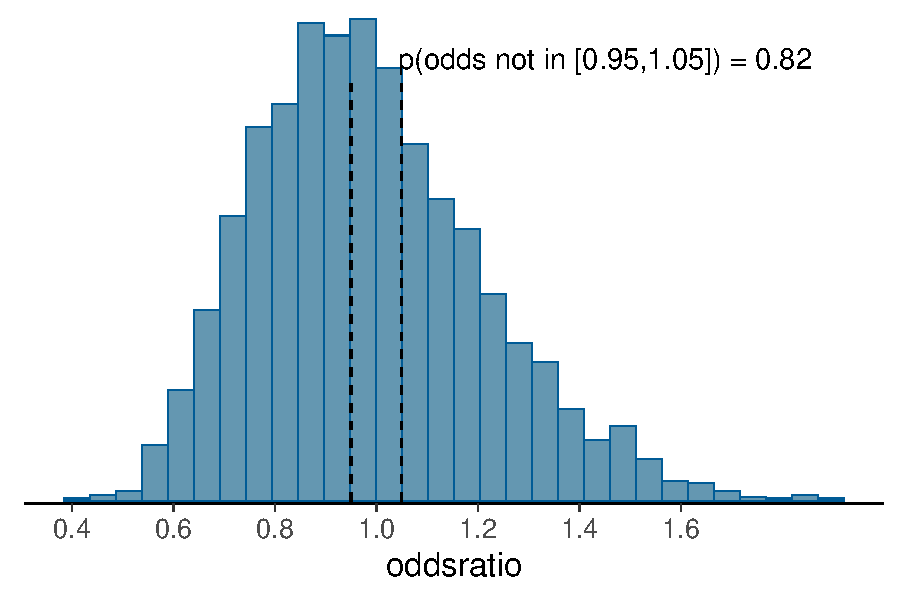
\includegraphics[width=6.8cm]{odds2_rope.pdf}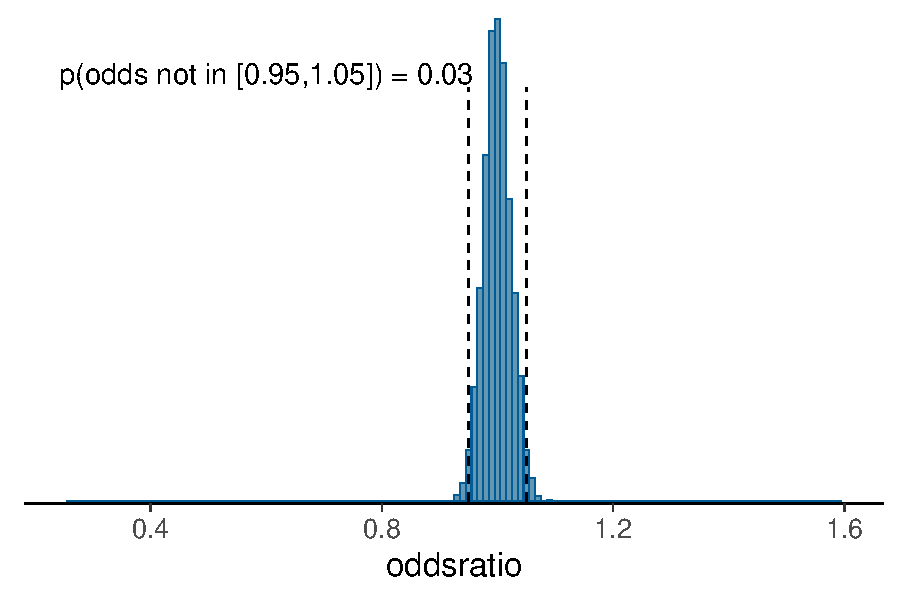
\includegraphics[width=6.8cm]{odds3_rope.pdf}
    \end{minipage}}
  \only<5>{\begin{minipage}{14.1cm}
      \hspace{-1.2cm}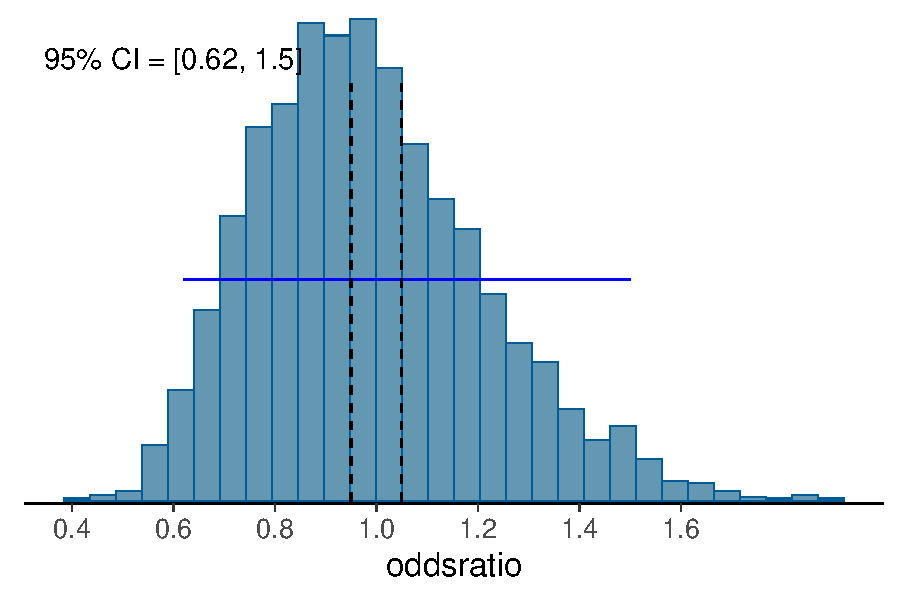
\includegraphics[width=6.8cm]{odds2_cirope.pdf}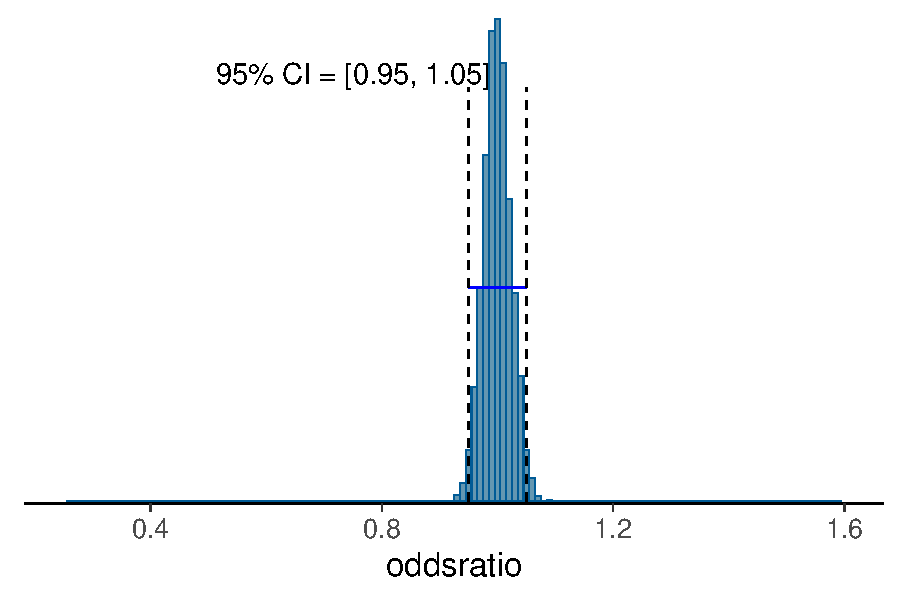
\includegraphics[width=6.8cm]{odds3_cirope.pdf}
    \end{minipage}}
  
\end{frame}

\begin{frame}{Bayesian hypothesis testing}

  \begin{itemize}
  \item Bayes factor
    \begin{itemize}
    \item null model has, e.g., the treatment effect fixed to 0
    \item assumes that there is non-zero probability that the
      treatment effect can be exactly zero (point mass)
    \item requires posterior inference for the null model, too
    \end{itemize}
  \end{itemize}
    \vspace{-1\baselineskip}
  
    \only<1>{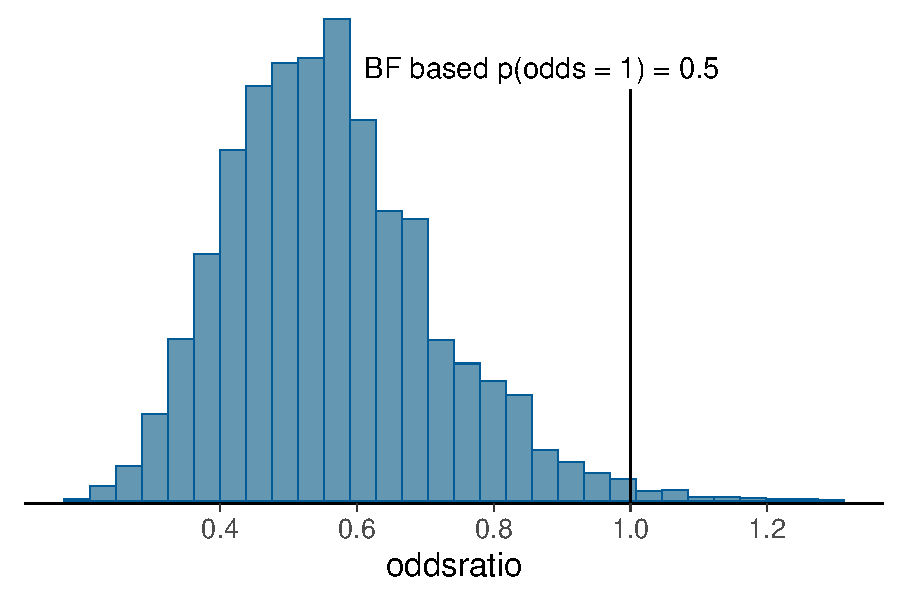
\includegraphics[width=9cm]{odds1_bf.pdf}}
    \only<2>{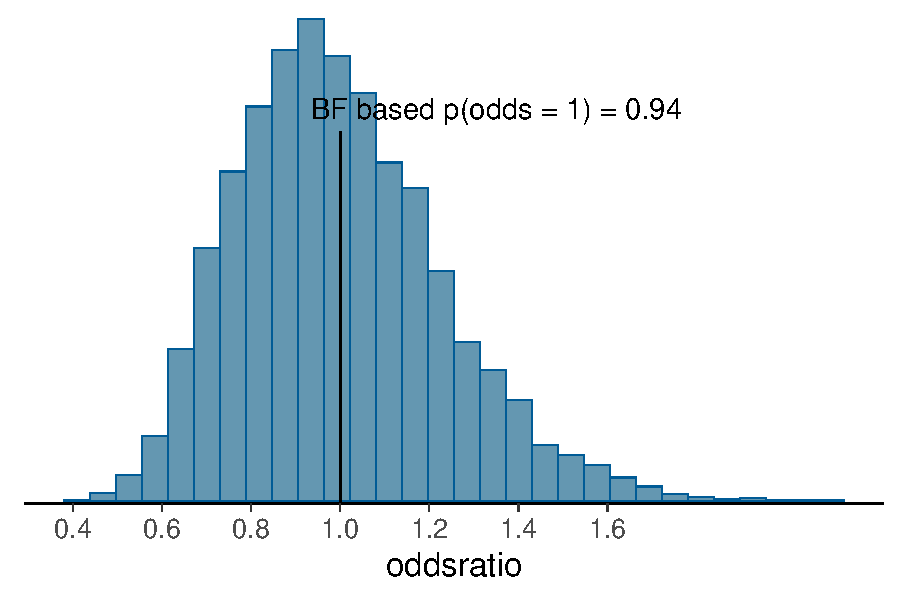
\includegraphics[width=9cm]{odds2_bf.pdf}}
    \only<3>{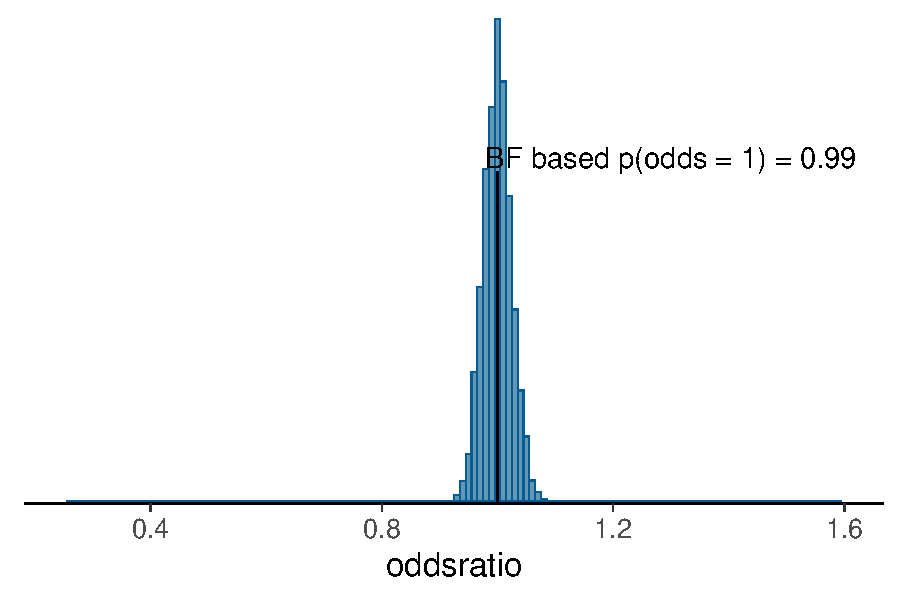
\includegraphics[width=9cm]{odds3_bf.pdf}}
    \vspace{-1.2\baselineskip}
    
    {\footnotesize\color{gray}\hspace{1cm}  with {\tt bridgesampling} package, see also BDA3 13.10}
\end{frame}

\begin{frame}{Bayesian hypothesis testing}

  \begin{itemize}
  \item Bayes factor
    \begin{itemize}
    \item sensitive to the prior choice even when the posterior is not
    \end{itemize}
  \end{itemize}
  normal(0,3.5) \hspace{4.5cm} normal(0,100)
  \begin{minipage}{14.1cm}
      \hspace{-1.2cm}{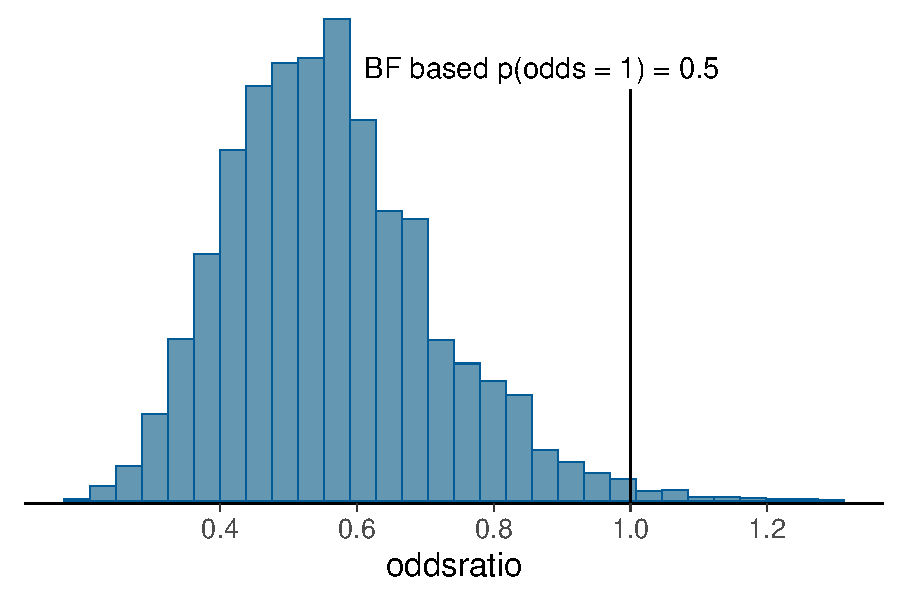
\includegraphics[width=6.8cm]{odds1_bf.pdf}}{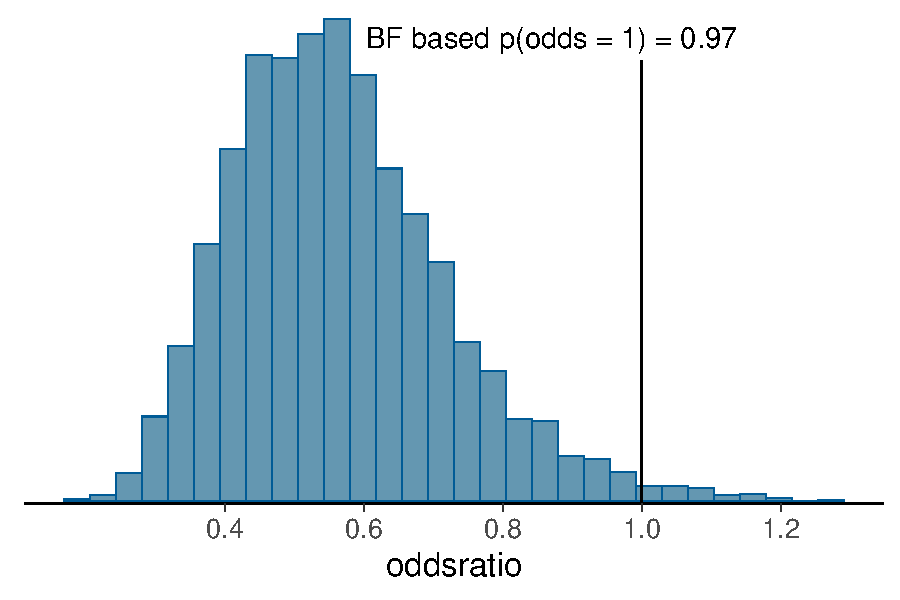
\includegraphics[width=6.8cm]{odds1_bf100.pdf}}
    \end{minipage}
      \vspace{-1.2\baselineskip}
    {\footnotesize\color{gray}\hspace{1cm}  with {\tt bridgesampling} package, see also BDA3 13.10}
\end{frame}

\begin{frame}{Bayesian hypothesis testing}

  \begin{itemize}
  \item Predictive performance
    \begin{itemize}
    \item is there difference in predictive performance with, e.g.,
      treatment effect fixed to zero or unknown treatment effect
    \item requires posterior inference for the null model or
      projection from the full to null
    \item looking at the posterior is better if parameters are
      independent
    \end{itemize}
  \end{itemize}

  \uncover<2->{
  In the beta blockers example
  \begin{itemize}
  \item Leave-one-person-out works, but is less efficient than looking
    at the posterior (see
    \url{https://avehtari.github.io/modelselection/betablockers.html})
  \end{itemize}
}

\end{frame}


\begin{frame}{Simulation experiment}

  \vspace{-0.75\baselineskip}
  
  \begin{minipage}{3.2cm}
    \vspace{-4\baselineskip}
    \hfill p(odds < 1)
  \end{minipage}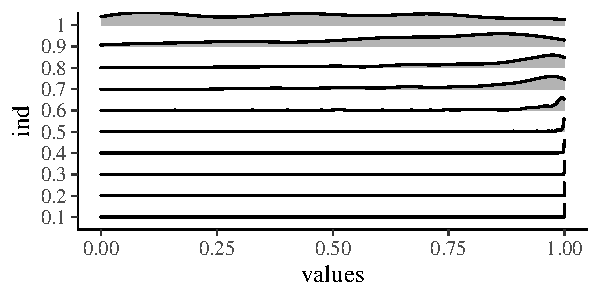
\includegraphics[width=6cm]{simuridges_beta.pdf}
\uncover<2->{  
  \begin{minipage}{3.2cm}
    \vspace{-4\baselineskip}
    \hfill Marginal likelihood comparison
  \end{minipage}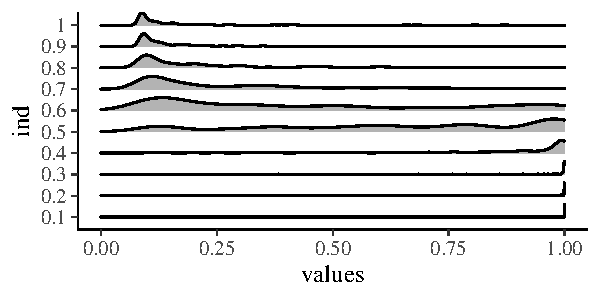
\includegraphics[width=6cm]{simuridges_bf.pdf}
  }
\uncover<3->{  
  \vspace{-1\baselineskip}
  
  \begin{minipage}{3.2cm}
    \vspace{-4\baselineskip}
    \hfill LOO comparison
  \end{minipage}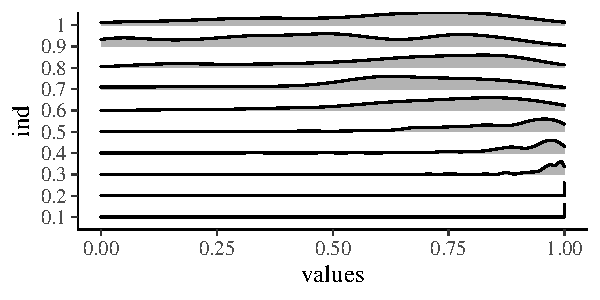
\includegraphics[width=6cm]{simuridges_loo.pdf}
  \vspace{-1\baselineskip}
  }
  
\end{frame}

\begin{frame}{Hypothesis testing and posterior dependencies}

  \vspace{-0.5\baselineskip}
  Looking at the marginal posterior $p(\beta < 0)$ can be misleading when there
  are many parameters
  
  Marginal posteriors of coefficients
  
  \includegraphics[width=10cm]{bodyfat_mcmc_areas.pdf}

\end{frame}

\begin{frame}{Hypothesis testing and posterior dependencies}

  \vspace{-0.75\baselineskip}
  Looking at the marginal posterior(s) can be misleading when there
  are many parameters

  Bivariate marginal of weight and height
  
  \vspace{-0.25\baselineskip}
  \includegraphics[width=6.8cm]{bodyfat_mcmc_scatter.pdf}

\end{frame}


\begin{frame}{Hypothesis testing and posterior dependencies}

  In bodyfat example, starting from full model

  \begin{itemize}
  \item BF in favor of removing weight (p=0.92)
  \item LOO in favor of removing weight (p=0.99)
  \end{itemize}

  In bodyfat example, starting from model y $\sim$ abdomen
  \begin{itemize}
  \item BF in favor of adding weight (p=1.0)
  \item LOO in favor of adding weight (p=1.0)
  \end{itemize}

\end{frame}

\begin{frame}{Variable selection}

  \vspace{-0.5\baselineskip}
  More elaborate approaches are needed for variable selection

  Projection predictive variable selection selects the minimal set of
  variables with similar predictive performance as the full model
  
  \includegraphics[width=10cm]{bodyfat_varsel_plot.pdf}

\end{frame}


\end{document}

%%% Local Variables: 
%%% TeX-PDF-mode: t
%%% TeX-master: t
%%% End: 
